% Microtissue between pillars: top view of the three gel patches and twelve pillars, section of a pillar (lid on the gel).
% Build: pdflatex hill_microtissue_pillars_bcs.tex && pdftocairo -svg hill_microtissue_pillars_bcs.pdf hill_microtissue_pillars_bcs.svg
\documentclass[tikz,border=4pt]{standalone}
\usetikzlibrary{arrows.meta,patterns,calc}
\tikzset{
	edge/.style={thick},
	gel/.style={fill=cyan!10},
	core/.style={fill=cyan!22},
	pillar/.style={fill=gray!45,draw=black},
	clamp/.style={pattern=north east lines,pattern color=red!60!black},
	roi/.style={draw=orange!80!black,thick,dashed},
	cut/.style={draw=blue!60!black,very thick,dash pattern=on 4pt off 2pt},
	ax/.style={-{Latex[length=2mm]}},
	dim/.style={{Latex[length=1.6mm]}-{Latex[length=1.6mm]},thin},
}
\begin{document}
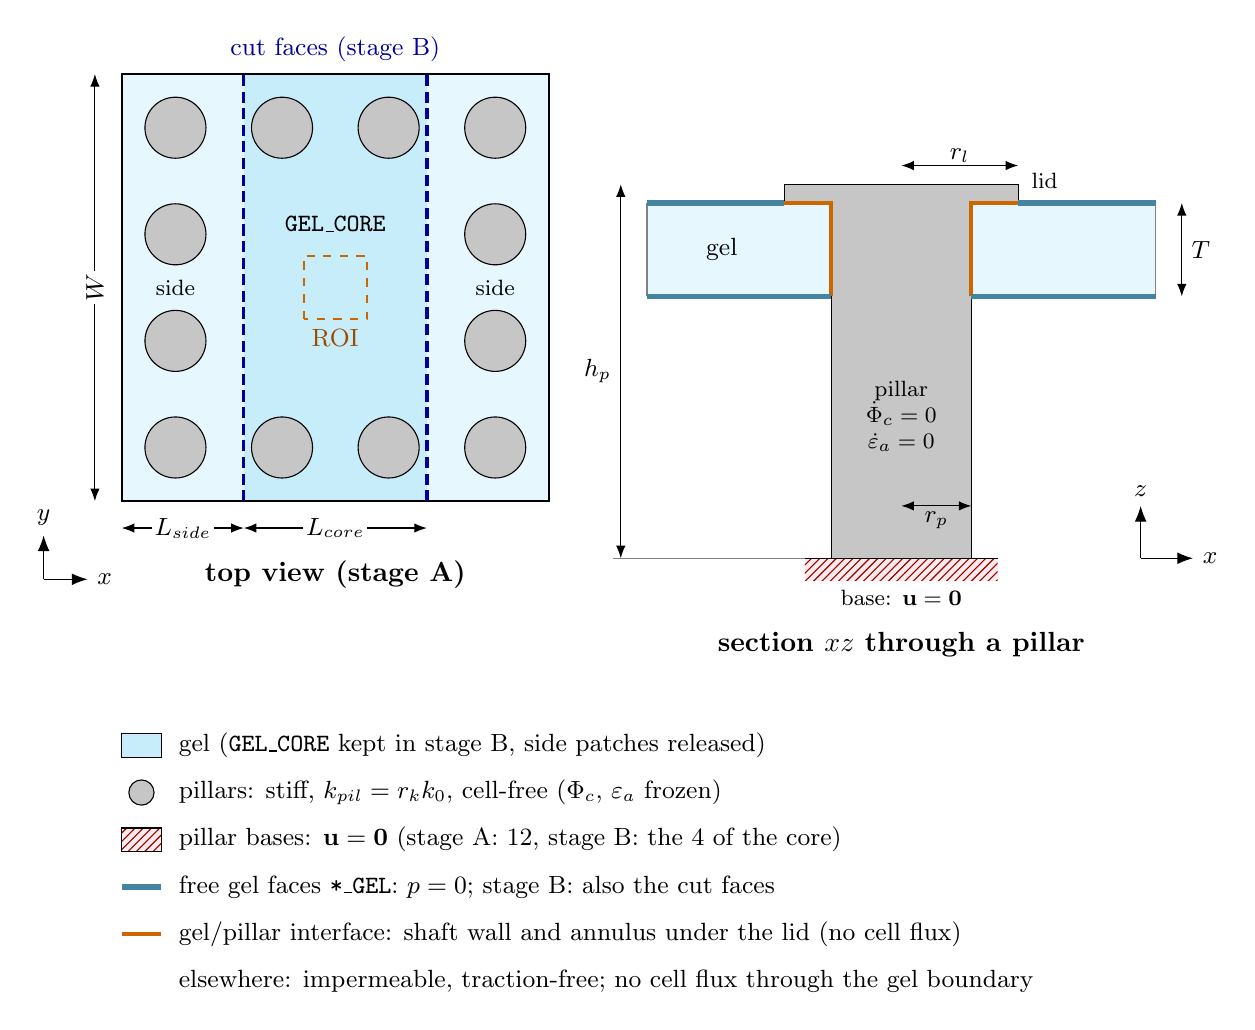
\begin{tikzpicture}[font=\small]
	% ---------------- top view, 1 unit = 100 um ----------------
	\begin{scope}[scale=0.62]
		\def\Lx{8.75}\def\W{8.75}\def\Ls{2.5}\def\Lc{3.75}\def\m{1.1}\def\s{2.1833}\def\rl{0.625}
		\fill[gel] (0,0) rectangle (\Ls,\W); \fill[core] (\Ls,0) rectangle (\Ls+\Lc,\W);
		\fill[gel] (\Ls+\Lc,0) rectangle (\Lx,\W);
		\draw[edge] (0,0) rectangle (\Lx,\W);
		\draw[cut] (\Ls,0) -- (\Ls,\W) (\Ls+\Lc,0) -- (\Ls+\Lc,\W);
		% twelve pillars (lids), core ones on the front/back edges
		\foreach \x/\y in {\m/\m, \m/\m+\s, \m/\W-\m-\s, \m/\W-\m, \Lx-\m/\m, \Lx-\m/\m+\s, \Lx-\m/\W-\m-\s, \Lx-\m/\W-\m,
				\m+\s/\m, \Lx-\m-\s/\m, \m+\s/\W-\m, \Lx-\m-\s/\W-\m}
			\filldraw[pillar] (\x,\y) circle (\rl);
		% region of interest (post-processing), 130 um square at the centre
		\draw[roi] (\Lx/2-0.65,\W/2-0.65) rectangle (\Lx/2+0.65,\W/2+0.65);
		\node[orange!60!black,below] at (\Lx/2,\W/2-0.65) {ROI};
		% labels
		\node[font=\footnotesize] at (\m,\W/2) {side};
		\node at (\Ls+\Lc/2,\W/2+1.3) {\texttt{GEL\_CORE}};
		\node[font=\footnotesize] at (\Lx-\m,\W/2) {side};
		\node[blue!60!black,above] at (\Ls+\Lc/2,\W+0.05) {cut faces (stage B)};
		\draw[dim] (0,-0.55) -- node[fill=white,inner sep=1pt] {$L_{side}$} (\Ls,-0.55);
		\draw[dim] (\Ls,-0.55) -- node[fill=white,inner sep=1pt] {$L_{core}$} (\Ls+\Lc,-0.55);
		\draw[dim] (-0.55,0) -- node[fill=white,inner sep=1pt,rotate=90] {$W$} (-0.55,\W);
		% axes
		\begin{scope}[shift={(-1.6,-1.6)}]
			\draw[ax] (0,0) -- (0.9,0) node[right] {$x$};
			\draw[ax] (0,0) -- (0,0.9) node[above] {$y$};
		\end{scope}
		\node[font=\bfseries] at (\Lx/2,-1.5) {top view (stage A)};
	\end{scope}

	% ---------------- side section through a pillar, 1 unit = 40 um ----------------
	\begin{scope}[shift={(9.9,2.6)},scale=0.95]
		\def\T{1.25}\def\rp{0.9375}\def\rl{1.5625}\def\tl{0.25}\def\hp{5}\def\half{3.4}\def\zb{-3.5}% z_b = T + t_l - h_p
		% gel slab around the pillar
		\fill[gel] (-\half,0) rectangle (\half,\T);
		\draw[edge] (-\half,0) -- (\half,0) (-\half,\T) -- (\half,\T);
		\draw[thin,gray] (-\half,0) -- (-\half,\T) (\half,0) -- (\half,\T);
		% pillar: leg + shaft (radius r_p) from the base z_b to the gel top z = T, lid (radius r_l) on top of the gel
		\filldraw[pillar] (-\rp,\zb) -- (-\rp,\T) -- (-\rl,\T) -- (-\rl,\T+\tl) -- (\rl,\T+\tl) -- (\rl,\T)
			-- (\rp,\T) -- (\rp,\zb) -- cycle;
		% gel/pillar interface (SIDE_PILLARS): shaft wall in the gel and annulus under the lid
		\draw[orange!80!black,line width=1.4pt] (-\rp,0) -- (-\rp,\T) -- (-\rl,\T) (\rp,0) -- (\rp,\T) -- (\rl,\T);
		% clamped base
		\fill[red!8] (-\rp-0.35,\zb-0.3) rectangle (\rp+0.35,\zb);
		\fill[clamp] (-\rp-0.35,\zb-0.3) rectangle (\rp+0.35,\zb);
		\draw (-\rp-0.35,\zb) -- (\rp+0.35,\zb);
		% drained gel faces
		\foreach \xa/\xb in {-\half/-\rl, \rl/\half} \draw[cyan!60!black,line width=2pt] (\xa,\T) -- (\xb,\T);
		\foreach \xa/\xb in {-\half/-\rp, \rp/\half} \draw[cyan!60!black,line width=2pt] (\xa,0) -- (\xb,0);
		% labels
		\node at (-2.4,\T/2) {gel};
		\node[align=center,font=\footnotesize] at (0,-1.6) {pillar\\$\dot\Phi_c = 0$\\$\dot\varepsilon_a = 0$};
		\node[right,font=\footnotesize] at (\rl+0.05,\T+0.3) {lid};
		\node[below,font=\footnotesize] at (0,\zb-0.3) {base: $\mathbf u = \mathbf 0$};
		\draw[dim] (\half+0.35,0) -- node[right] {$T$} (\half+0.35,\T);
		\draw[dim] (-\half-0.35,\T+\tl) -- node[left] {$h_p$} (-\half-0.35,\zb);
		\draw[thin,gray] (-\half-0.45,\zb) -- (-\rp-0.35,\zb);
		\draw[dim] (0,-2.8) -- node[below,inner sep=2pt] {$r_p$} (\rp,-2.8);
		\draw[dim] (0,\T+\tl+0.25) -- node[above,inner sep=1pt] {$r_l$} (\rl,\T+\tl+0.25);
		\node[font=\bfseries] at (0,\zb-1.15) {section $xz$ through a pillar};
		\begin{scope}[shift={(\half-0.2,\zb)}]
			\draw[ax] (0,0) -- (0.7,0) node[right] {$x$};
			\draw[ax] (0,0) -- (0,0.7) node[above] {$z$};
		\end{scope}
	\end{scope}

	% ---------------- legend ----------------
	\begin{scope}[shift={(0,-3.1)}]
		\fill[core] (0,-0.15) rectangle (0.5,0.15); \draw (0,-0.15) rectangle (0.5,0.15);
		\node[right] at (0.6,0) {gel (\texttt{GEL\_CORE} kept in stage B, side patches released)};
		\filldraw[pillar] (0.25,-0.6) circle (0.16);
		\node[right] at (0.6,-0.6) {pillars: stiff, $k_{pil} = r_k k_0$, cell-free ($\Phi_c$, $\varepsilon_a$ frozen)};
		\fill[red!8] (0,-1.35) rectangle (0.5,-1.05); \fill[clamp] (0,-1.35) rectangle (0.5,-1.05);
		\draw (0,-1.35) rectangle (0.5,-1.05);
		\node[right] at (0.6,-1.2) {pillar bases: $\mathbf u = \mathbf 0$ (stage A: 12, stage B: the 4 of the core)};
		\draw[cyan!60!black,line width=2pt] (0,-1.8) -- (0.5,-1.8);
		\node[right] at (0.6,-1.8) {free gel faces \texttt{*\_GEL}: $p = 0$; stage B: also the cut faces};
		\draw[orange!80!black,line width=1.4pt] (0,-2.4) -- (0.5,-2.4);
		\node[right] at (0.6,-2.4) {gel/pillar interface: shaft wall and annulus under the lid (no cell flux)};
		\node[right] at (0.6,-3.0) {elsewhere: impermeable, traction-free; no cell flux through the gel boundary};
	\end{scope}
\end{tikzpicture}
\end{document}
